\section{Benchmarking}

Kernkonzept nutzt eine zu großen Teilen intern entwickelte Pipeline zur
automatisierten Ausführung von Integrations-Tests und Benchmark-Programmen
auf verschiedenen Hardware-Plattformen.
Die gesammelten Benchmark-Ergebnisse werden auf einem zentralen Server
gespeichert und können über ein Web-Frontend dargestellt werden.

Das bisherige Frontend ist hauptsächlich in Perl 5 und JavaScript
geschriebenen. Es erfüllt seinen Zweck, ist aber in manchen Belangen nicht
flexibel genug. Vor allem ist das Einbinden neuer Funktionen teilweise mit
größerem Aufwand verbunden und nur mit ausreichender Kenntnis der
existierenden Software möglich.

Es wurde die Nutzung von \textit{Jupyter} als Alternative evaluiert. Jupyter
ist in Web-Frontend für den \textit{IPython} Kernel (unter anderen) und erlaubt
die Ausführung von Python-Code in einem Zellen-basierten Editor im Browser. In
den so entwickelten sogenannten Notebooks lassen sich neben Python-Code auch
mit gängigen Plotting-Bibliotheken erzeugte Grafiken inline darstellen. Die
Ergebnisse können dann beispielsweise automatisch in verschiedene Formate
exportiert werden, die gängige Browser auch ohne Jupyter Installation
darstellen können.

Die Umstellung der Benchmark-Daten-Visualisierung auf Jupyter bringt vor allem
einen Vorteil mit sich: Es existieren aufgrund der Beliebtheit von Python in
der Data Science Community etliche aktiv entwickelte Open Source Bibliotheken
zur statistischen Analyse und Darstellung von Daten. Dies kann in Zukunft die
Implementierung von spezialisierten Funktionalitäten ersparen, für die die
beispielsweise bereits eine verfügbare Python- aber keine äquivalente
JavaScript-Lösung existiert.

\subsection{Datenanfrage}

Zunächst wurde ein Teil des existierenden Perl 5 Codes, der für die Abfrage der
Benchmark-Daten vom Server verantwortlich ist, nach Python portiert.  Die
Benchmark-Daten werden auf einem Test-Server von in festgelegten Intervallen
geschedulten Jobs erzeugt.  Diese führen teilweise komplexe Integrations-Tests
aus und messen verschiedene Performance-Metriken, z.B. Latenzen beim Versenden
von IP-Paketen zwischen verschiedenen VM Instanzen.

Für die strukturierte Speicherung und Verwaltung dieser Metriken existieren
verschiedene Backend-Implementierungen, u.a. RDBMS oder \textit{Elastisearch}
basiert.  Die Abfrage der Daten ist nach außen über ein JSON basiertes
Interface abstrahiert. Dieses ähnelt gebräuchlichen deklarativen
Anfragesprachen wie etwa SQL ist aber deutlich einfacher gehalten.

Die derart persistierten Daten können vom Server, auf dem sie abgelegt sind,
angefragt werden, indem eine Query im JSON Format per HTTP POST-Anfrage an den
Server übertragen wird. Die zur Anfrage passenden Daten sind in der HTTP
Antwort (im CSV Format) enthalten.

\subsection{Visualisierung}

Um die angefragten Daten darzustellen, wurde eine Python Bibliothek geschrieben,
die häufig anfallende Visualisierungs-Aufgaben einfach macht.  Diese ermöglicht
die direkte Darstellung von Histogrammen, Boxplots, Quantilen etc. direkt mit
den in Python-Objekten gekapselten angefragten Datensätzen. Die Bibliothek
nutzt dabei die Python Plotting Bibliotheken \textit{Matplotlib} und
\textit{Bokeh} als austauschbare Backends und abstrahiert über deren
unterschiedliche APIs. Bokeh erzeugt mittels JavaScript-Generierung interaktive
Plots (mit integrierter Zoom-Funktion usw.), was diese besonders gut in aus
Jupyter Notebooks erzeugten Web-Dokumenten nutzbar macht. Das Matplotlib
Backend wurde zusätzlich implementiert, da Bokeh sich noch in einer frühen
Entwicklungsphase befindet und vor allem bezüglich Dokumentation und
API-Stabilität weniger ausgereift ist. Technisch war hier die sinnvolle
Abstrahierung und Konsolidierung der teilweise sehr ,,grundlegenden'' von Bokeh
und Matplotlib angebotenen Plotting-Funktionen zu einem für den vorliegenden
Anwendungsfall geeigneten ,,high-level'' Interface eine Herausforderung.

\subsection{Regelkarten}

\textit{Regelkarte} ist ein Oberbegriff für verschiedene statistische Methoden,
die genutzt werden können um das ,,Außer-Kontrolle-Geraten'' eines
statistischen Schwankungen unterliegenden Prozesses zu erkennen. Man stelle
sich als Beispiel eine in regelmäßigen Zeitabständen gemessene L4Re
Performance-Metrik vor (zum Beispiel Latenz einer bestimmten Form der
Netzwerk-Kommunikation), für die der ermittelte Wert im Normalfall ungefähr um
einen konstanten Mittelwert normalverteilt ist. Es wäre nun wünschenswert, es
ohne manuelle Inspektion zu ermöglichen, Abweichung von diesem Verhalten, wie
zum Beispiel eine Verschiebung des Mittelwertes, rechtzeitig zu erkennen und
auf gewisse Commits zurückführen zu können. Eine naive Lösung wäre es, einen
cron-Job o.ä. anzulegen, der nach jeder Messung eine Warnung ausgibt, wenn die
ermittelte Metrik einen festen Grenzwert überschreitet. Dies führt dann aber in
den meisten Fällen entweder zu vielen Falschmeldungen, wenn der Grenzwert zu
eng angesetzt ist oder andernfalls zu später (oder gar keiner) Erkennung von
anhaltenden, aber kleinen Abweichungen im Mittelwert oder der
Standardabweichung des Prozesses.

Verschiedene Regelkarten können hier Abhilfe schaffen. Die meisten von ihnen
setzen normalverteilte Prozesse mit bekanntem Mittelwert und Standardabweichung
voraus (die aber auch aus einer Menge von Datenpunkten mit statistischen
Formeln angenähert werden können) und berechnen aus einer Zeitreihe von
Messwerten kumulativ einen Wert, der als Maß für das Außer-Kontrolle-Geraten
des Prozesses genutzt und auf Überschreitung eines Grenzwertes geprüft werden
kann.

Bei \textit{CUSUM} Regelkarten werden so zum Beispiel die akkumulierten Differenzen
zwischen dem Prozess-Mittelwert und dem Sollwert betrachtet, wodurch auch
kleine systematisch Verschiebungen des Mittelwertes detektiert werden können.
Letztlich wurden die Regelkarten-Typen $\bar{x}$ \textit{and R}, $\bar{x}$
\textit{and s}, \textit{ImR}, \textit{XmR}, \textit{EWMA} und \textit{CUSUM} in
die Benchmark-Visualisierungs-Bibliothek aufgenommen. Die genaue
Auseinandersetzung mit einzelner Regelkarten übersteigt den Rahmen dieses
Berichtes, für eine für Nicht-Statistiker zugängliche Einführung in gängige
Regelkarten-Typen siehe~\cite{nist}.

Listing~\ref{lst:control_charts} zeigt Beispielhaft die Erzeugung einer Reihe von
Regelkarten. Per JSON werden hier die zu analysierenden Datenpunkte sowie
Regelkarten-Typen spezifiziert. Bei der Erzeugung der Regelkarten-Objekte werden
die Datenpunkte per HTTP Post-Anfrage an \texttt{TAGET\_BASE\_URL} von einem
Server abgefragt. Schließlich werden die Regelkarten visualisiert, das Ergebnis
zeigt Abbildung~\ref{fig:control_charts}. In diesem Fall ist der Prozess unter
Kontrolle, in allen Regelkarten wird der ,,Kontrollbereich'' (abgegrenzt durch
,,Upper'' und ,,Lower Control Limit'' (UCL und LCL)) nicht verlassen.

\begin{mintlisting}[label=lst:control_charts]{mintpython}{Regelkarten-Visualisierung}
json_data = {
    "TARGET_BASE_URL" : "http://.../api/v1/",
    "METRIC" : {
        "NAME": "l4re.bmk.memory.stream.scale",
        "REF_QUERY": {
           "where" : [["<=", "CREATED", "2018-04-13 00:00:00"]]
        },
        "MONITOR_BASENAME": "MONITOR.processcontrol.ct.stream.x201.l4linux.l4vio_net_p2p",
        "MONITOR_VERSION": 1001,
        "MONITOR_QUERY": {
            "where" : [["=", "l4re_platform_hwcodename", "PCX201A"]]
        },
        "MONITOR_PARAMS" : {},
        "MONITOR_TYPES": [
            "cusum",
            "ewma",
            "xbar_s"
        ],
        "MONITOR_START": "2018-04-01 00:00:01",
        "SUBGROUP_SIZE": 5
    }
}

# create control charts
xbar_s = ControlChart.from_json('xbar_s', json_data)
cusum = ControlChart.from_json('cusum', json_data)
ewma = ControlChart.from_json('ewma', json_data)

# plot control charts
vis = MatplotlibPlotter()

vis.start()
vis.xbar_s(xbar_s, equidistant=True)
vis.cusum(cusum, equidistant=True)
vis.ewma(ewma, equidistant=True)
vis.show()
\end{mintlisting}

\begin{figure}
  \centering
  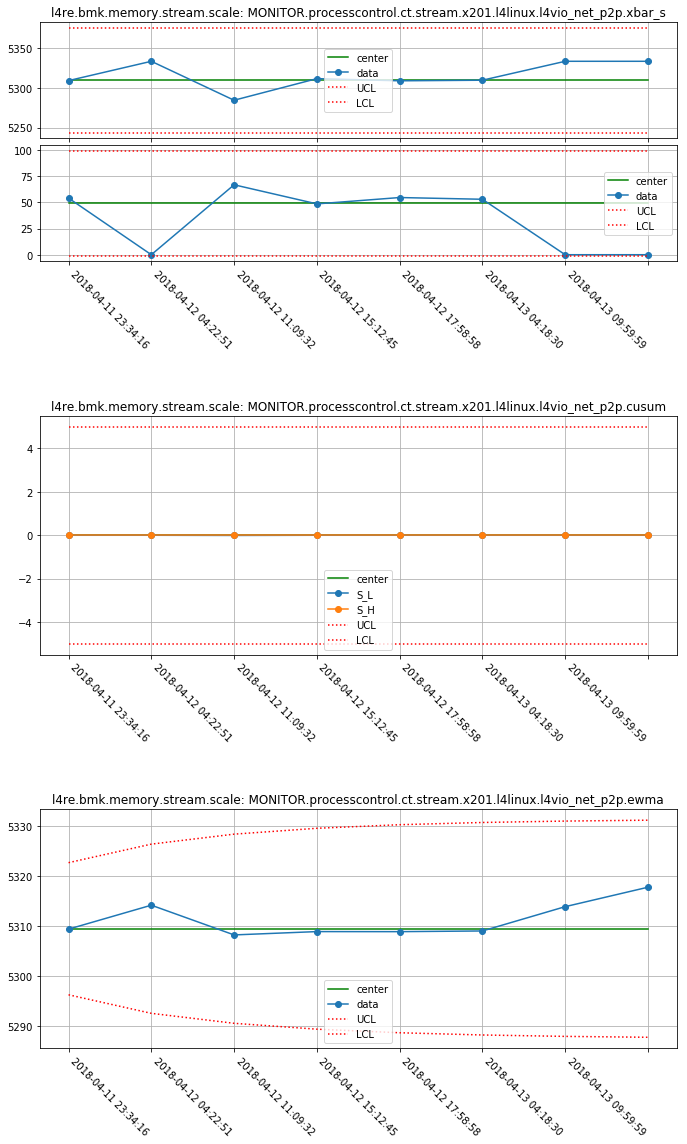
\includegraphics[scale=.6]{../resources/control_charts.png}
  \caption{Regelkarten-Visualisierung}
  \label{fig:control_charts}
\end{figure}

Es wurde zusätzlich ein Python Skript geschrieben, das in regelmäßigen
Abständen die Verfügbarkeit neuer Datenpunkte verschiedener Metriken abfragt,
aus diesen und vorherigen Datenpunkte den nächsten Regelkarten Wert
berechnet, diesen in derselben Datenbank ablegt und bei detektierter Ausartung
des Prozesses eine definierbare Aktion ausführt (sinnvollerweise das
Verschicken einer warnenden Mail).
